\section*{Question 3}
    \subsection*{a)}
    The following figure will show the schedule for the virtual machines and their local task sets when using the \textit{Deadline Monotonic} scheduling algorithm locally and globally. When scheduling globally I assume that the deadline, which is used to determine priority, is equal to the period of the VM interface.\\
    \begin{figure}[H]
        \centering
        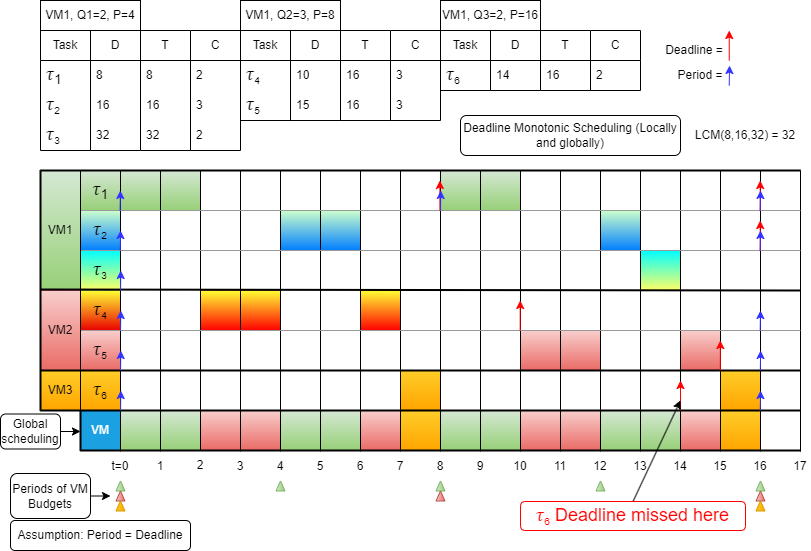
\includegraphics[width=0.6\textwidth]{images/AssQ3a.png}
        \caption{Schedule for the virtual machines and their local task sets when using the \textit{Deadline Monotonic} scheduling algorithm locally and globally.}
        \label{fig:3a}
    \end{figure}
    As we can see in figure \ref{fig:3a} the deadline of $\tau_6$ is missed at $t=14$. 

    \subsection*{b)}
    The following figure will show the schedule for the virtual machines and their local task sets when using the \textit{Earliest Deadline First} scheduling algorithm globally, but still \textit{Deadline Monotonic} locally. When scheduling globally I still assume that the deadline, which is used to determine priority, is equal to the period of the VM interface.\\

    \begin{figure}[H]
        \centering
        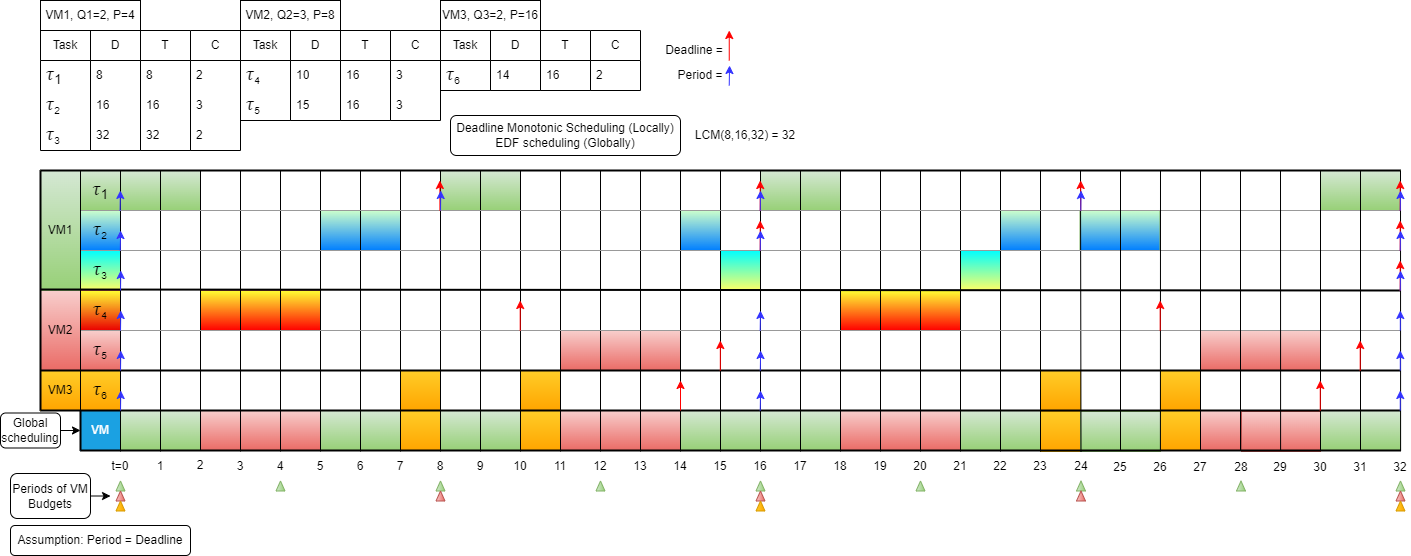
\includegraphics[width=1\textwidth]{images/AssQ3b.png}
        \caption{Schedule for the virtual machines and their local task sets when using the \textit{Earliest Deadline First} scheduling algorithm globally, but still \textit{Deadline Monotonic} locally.}
        \label{fig:3b}
    \end{figure}
    As we can see in figure \ref{fig:3b} all deadlines are met both globally and locally.

    \subsection*{c)}
    There are a few things that can be done, for example we can follow the example above of trying different scheduling algorithms, locally and globally, and analyse the traces to find the best option for that specific case. What more can be done is to use offsets when scheduling tasks. This can mitigate missing deadlines when loads are high, especially for lower priority tasks. So, in our example in question \textit{a} it could be a good idea to use offsets to give room for $\tau_6$ to execute.